\subsection{Sort}\label{sec:sort}

We implemented a generic module, SortModule, that sorts the records in a DataSeries file. The name of the sorting field (ie, key field) and the ``comparator'' function must be specified. SortModule attempts to sort all the records in memory. If the file is larger than the available memory, SortModule performs an external sort.

For the experiment, we created three files using the gensort utility of the TeraSort benchmark: 100 MiB (1000000 records), 1 GiB (10000000 records) and 10 GiB (100000000 records). For each of the three datasets, we created three DataSeries files: one without compression, one with lzf compression and one with gzip compression.

We expected the 100 MB and 1 GB files to sort entirely in main memory, and the 10 GB file to require an external sort. An external sort involves writing temporary sorted files to disk and then merging those files to create the final sorted output. When running the analysis program on the 10 GB files, we experimented with lzf compression for the intermediate files. (We only experimented with lzf for this purpose, because we needed an algorithm that has high throughput for both compression and decompression.) Since the throughput of the sort analysis was much lower than the available disk throughput, lzf compression hardly made a difference.

On the 1 GB files, the effective throughput of the analysis program was 16.45 MiB/s, 18.19 MiB/s and 19.98 MiB/s for the uncompressed file, the lzf-compressed file and the gzip-compressed file, respectively.

\subsubsection{Conversion to DataSeries}

The conversion to DataSeries was straightforward. We implemented a simple utility, gensort2txt, which convers a gensort-generated file to a DataSeries file by creating one record for each record of the binary file. The record consists of a two fixed-width fields: a 10-byte key and a 90-byte value. For lzf and gzip, we used the default compression settings of DataSeries.

Table~\ref{table:sort:compression} shows the sizes of each of the datasets in four different formats: the original gensort file, the uncompressed DataSeries format, the lzf DataSeries format and the gzip DataSeries format.


\begin{table*}
\centering
\begin{tabular}{|l|r|r|r|}\hline

Dataset    & 1000000 records & 10000000 records  & 100000000 records \\
\hline
Gensort             & 100.00 & 1000.00 & 10000.00 \\
none                & 104.11 & 1041.08 & 10410.79 \\
lzf                 & 41.73  & 417.33  & 4173.41  \\
gzip                & 27.33  & 273.34  & 2733.43  \\
\hline
\end{tabular}


\caption{File sizes (MiB) for the three datasets using different compression algorithms. Although the 10-byte keys are random (and, thus, not compressable), the 90-byte values are not random so they are compressable.}

\label{table:sort:compression}
\end{table*}

\subsubsection{Experiments}

For each of the datasets, we ran our analysis program on each of the three DataSeries formats (no compression, lzf and gzip). Table~\ref{table:sort:runtime} shows the runtime of these experiments. 
Compared to the grep analysis, compression had a limited effect on the throughput of the sort analysis. In fact, as the size of the dataset increases (from 100 MiB to 1 GiB to 10 GiB), reading/writing from/to disk consumes a smaller portion of the overall analysis time (because the sort algorithm itself, unlike the disk I/O, is not linear in the dataset size). Using lzf compression on the intermediate files of the external sort (for the 10 GiB dataset) actually reduced the throughput because it took valuable CPU cycles away from the sorting and merging.

Figure~\ref{fig:sort:throughput} shows the effective throughput for each of the experiments. The highest throughput achieved via compression was 1.24$\times$, 1.21$\times$ and 1.07$\times$ the throughput achieved without compression for the 100 MiB, 1 GiB and 10 GiB datasets, respectively.

\begin{table*}
\centering
\begin{tabular}{|l|r|r|r|}\hline

Dataset    & 100 MiB & 1 GiB  & 10 GiB \\
\hline
none/none   & 3.47  & 60.78  & 1116.85 \\
none/lzf    &       &        & 1149.74 \\
lzf/none    & 2.80  & 54.98  & 1052.67 \\
lzf/lzf     &       &        & 1131.92 \\
gzip/none   & 2.84  & 50.05  & 1046.81 \\
gzip/lzf    &       &        & 1074.19 \\
\hline
\end{tabular}

\caption{Average runtime of sortanalysis. The datasets are named ``$c_1$/$c_2$'', where $c_1$ is the type of compression for the input data, and $c_2$ is the type of compression for the intermediate files that are used in external (ie, two-phase) sorts.}

\label{table:sort:runtime}
\end{table*}

\begin{figure}
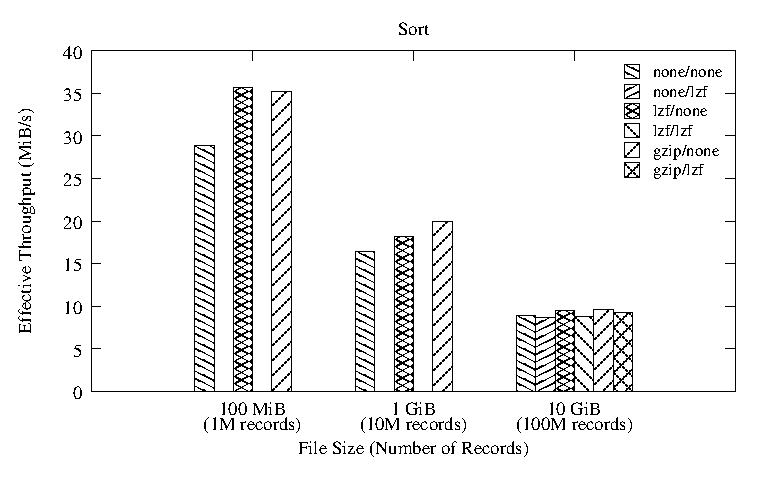
\epsfig{width=3.2in, angle=0, file=graphs/sort.ps}
\caption{Throughput of sorting 100-byte records with DataSeries using various compression algorithms (``gzip/lzf'' indicates that the input data was compressed with gzip, and the intermediate files of the external sort were compressed with lzf). Sorting is not linear in the amount of data, so increasing the number of records results in a lower throughput. Since the disk I/O needed for a sort is linear in the amount of data, compression makes less of a difference as the number of records increases. Furthermore, for the 10 GiB dataset that required an external (ie, two-phase) sort, compressing the intermediate files (via lzf) was not beneficial.}
\label{fig:sort:throughput}
\end{figure}


